% REV00 Tue 04 May 2021 13:55:16 WIB
% START Tue 04 May 2021 13:55:16 WIB

\chapter{XXX}

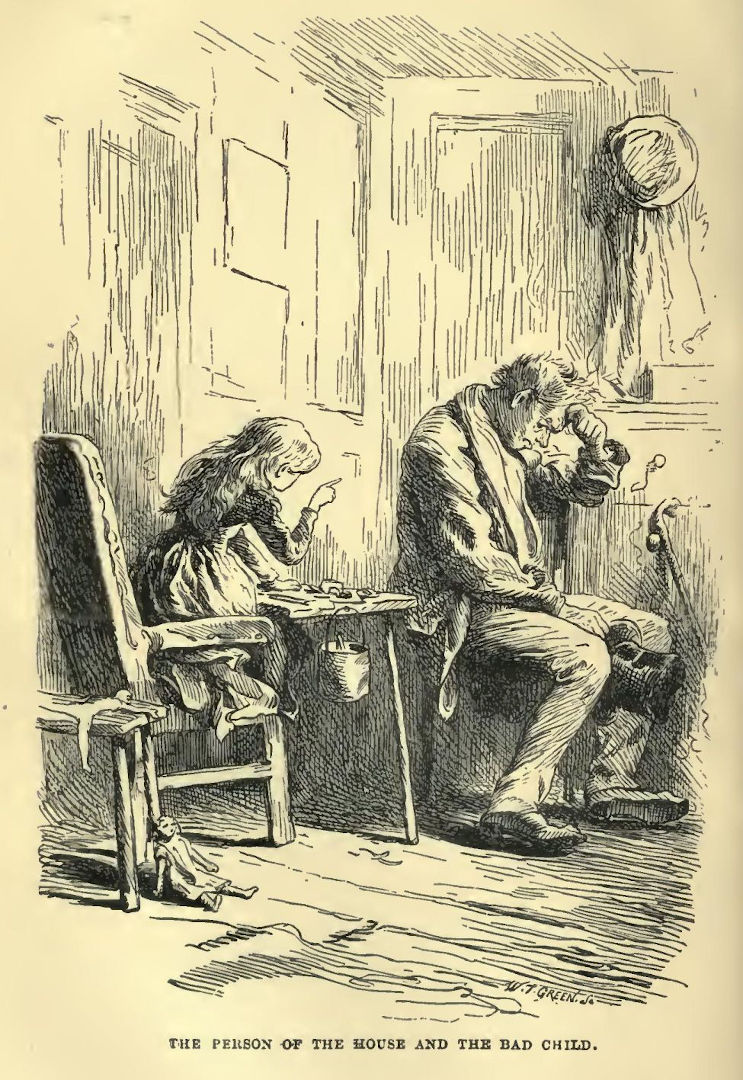
\includegraphics[scale=2.3]{02-02-01}

Chapter 15

THE WHOLE CASE SO FAR


Bradley Headstone held fast by that other interview he was to have with
Lizzie Hexam. In stipulating for it, he had been impelled by a feeling
little short of desperation, and the feeling abided by him. It was very
soon after his interview with the Secretary, that he and Charley Hexam
set out one leaden evening, not unnoticed by Miss Peecher, to have this
desperate interview accomplished.

‘That dolls’ dressmaker,’ said Bradley, ‘is favourable neither to me nor
to you, Hexam.’

‘A pert crooked little chit, Mr Headstone! I knew she would put herself
in the way, if she could, and would be sure to strike in with something
impertinent. It was on that account that I proposed our going to the
City to-night and meeting my sister.’

‘So I supposed,’ said Bradley, getting his gloves on his nervous hands
as he walked. ‘So I supposed.’

‘Nobody but my sister,’ pursued Charley, ‘would have found out such an
extraordinary companion. She has done it in a ridiculous fancy of giving
herself up to another. She told me so, that night when we went there.’

‘Why should she give herself up to the dressmaker?’ asked Bradley.

‘Oh!’ said the boy, colouring. ‘One of her romantic ideas! I tried to
convince her so, but I didn’t succeed. However, what we have got to do,
is, to succeed to-night, Mr Headstone, and then all the rest follows.’

‘You are still sanguine, Hexam.’

‘Certainly I am, sir. Why, we have everything on our side.’

‘Except your sister, perhaps,’ thought Bradley. But he only gloomily
thought it, and said nothing.

‘Everything on our side,’ repeated the boy with boyish confidence.
‘Respectability, an excellent connexion for me, common sense,
everything!’

‘To be sure, your sister has always shown herself a devoted sister,’
said Bradley, willing to sustain himself on even that low ground of
hope.

‘Naturally, Mr Headstone, I have a good deal of influence with her.
And now that you have honoured me with your confidence and spoken to me
first, I say again, we have everything on our side.’

And Bradley thought again, ‘Except your sister, perhaps.’

A grey dusty withered evening in London city has not a hopeful aspect.
The closed warehouses and offices have an air of death about them, and
the national dread of colour has an air of mourning. The towers and
steeples of the many house-encompassed churches, dark and dingy as the
sky that seems descending on them, are no relief to the general gloom;
a sun-dial on a church-wall has the look, in its useless black shade, of
having failed in its business enterprise and stopped payment for ever;
melancholy waifs and strays of housekeepers and porter sweep melancholy
waifs and strays of papers and pins into the kennels, and other more
melancholy waifs and strays explore them, searching and stooping and
poking for anything to sell. The set of humanity outward from the City
is as a set of prisoners departing from gaol, and dismal Newgate
seems quite as fit a stronghold for the mighty Lord Mayor as his own
state-dwelling.

On such an evening, when the city grit gets into the hair and eyes and
skin, and when the fallen leaves of the few unhappy city trees grind
down in corners under wheels of wind, the schoolmaster and the pupil
emerged upon the Leadenhall Street region, spying eastward for Lizzie.
Being something too soon in their arrival, they lurked at a corner,
waiting for her to appear. The best-looking among us will not look very
well, lurking at a corner, and Bradley came out of that disadvantage
very poorly indeed.

‘Here she comes, Mr Headstone! Let us go forward and meet her.’

As they advanced, she saw them coming, and seemed rather troubled. But
she greeted her brother with the usual warmth, and touched the extended
hand of Bradley.

‘Why, where are you going, Charley, dear?’ she asked him then.

‘Nowhere. We came on purpose to meet you.’

‘To meet me, Charley?’

‘Yes. We are going to walk with you. But don’t let us take the great
leading streets where every one walks, and we can’t hear ourselves
speak. Let us go by the quiet backways. Here’s a large paved court by
this church, and quiet, too. Let us go up here.’

‘But it’s not in the way, Charley.’

‘Yes it is,’ said the boy, petulantly. ‘It’s in my way, and my way is
yours.’

She had not released his hand, and, still holding it, looked at him with
a kind of appeal. He avoided her eyes, under pretence of saying, ‘Come
along, Mr Headstone.’ Bradley walked at his side--not at hers--and the
brother and sister walked hand in hand. The court brought them to a
churchyard; a paved square court, with a raised bank of earth about
breast high, in the middle, enclosed by iron rails. Here, conveniently
and healthfully elevated above the level of the living, were the dead,
and the tombstones; some of the latter droopingly inclined from the
perpendicular, as if they were ashamed of the lies they told.

They paced the whole of this place once, in a constrained and
uncomfortable manner, when the boy stopped and said:

‘Lizzie, Mr Headstone has something to say to you. I don’t wish to be an
interruption either to him or to you, and so I’ll go and take a little
stroll and come back. I know in a general way what Mr Headstone intends
to say, and I very highly approve of it, as I hope--and indeed I do
not doubt--you will. I needn’t tell you, Lizzie, that I am under great
obligations to Mr Headstone, and that I am very anxious for Mr Headstone
to succeed in all he undertakes. As I hope--and as, indeed, I don’t
doubt--you must be.’

‘Charley,’ returned his sister, detaining his hand as he withdrew it, ‘I
think you had better stay. I think Mr Headstone had better not say what
he thinks of saying.’

‘Why, how do you know what it is?’ returned the boy.

‘Perhaps I don’t, but--’

‘Perhaps you don’t? No, Liz, I should think not. If you knew what
it was, you would give me a very different answer. There; let go; be
sensible. I wonder you don’t remember that Mr Headstone is looking on.’

She allowed him to separate himself from her, and he, after saying, ‘Now
Liz, be a rational girl and a good sister,’ walked away. She remained
standing alone with Bradley Headstone, and it was not until she raised
her eyes, that he spoke.

‘I said,’ he began, ‘when I saw you last, that there was something
unexplained, which might perhaps influence you. I have come this evening
to explain it. I hope you will not judge of me by my hesitating manner
when I speak to you. You see me at my greatest disadvantage. It is most
unfortunate for me that I wish you to see me at my best, and that I know
you see me at my worst.’

She moved slowly on when he paused, and he moved slowly on beside her.

‘It seems egotistical to begin by saying so much about myself,’ he
resumed, ‘but whatever I say to you seems, even in my own ears, below
what I want to say, and different from what I want to say. I can’t help
it. So it is. You are the ruin of me.’

She started at the passionate sound of the last words, and at the
passionate action of his hands, with which they were accompanied.

‘Yes! you are the ruin--the ruin--the ruin--of me. I have no resources
in myself, I have no confidence in myself, I have no government of
myself when you are near me or in my thoughts. And you are always in my
thoughts now. I have never been quit of you since I first saw you. Oh,
that was a wretched day for me! That was a wretched, miserable day!’

A touch of pity for him mingled with her dislike of him, and she said:
‘Mr Headstone, I am grieved to have done you any harm, but I have never
meant it.’

‘There!’ he cried, despairingly. ‘Now, I seem to have reproached you,
instead of revealing to you the state of my own mind! Bear with me. I am
always wrong when you are in question. It is my doom.’

Struggling with himself, and by times looking up at the deserted windows
of the houses as if there could be anything written in their grimy panes
that would help him, he paced the whole pavement at her side, before he
spoke again.

‘I must try to give expression to what is in my mind; it shall and must
be spoken. Though you see me so confounded--though you strike me so
helpless--I ask you to believe that there are many people who think well
of me; that there are some people who highly esteem me; that I have in
my way won a Station which is considered worth winning.’

‘Surely, Mr Headstone, I do believe it. Surely I have always known it
from Charley.’

‘I ask you to believe that if I were to offer my home such as it is, my
station such as it is, my affections such as they are, to any one of the
best considered, and best qualified, and most distinguished, among the
young women engaged in my calling, they would probably be accepted. Even
readily accepted.’

‘I do not doubt it,’ said Lizzie, with her eyes upon the ground.

‘I have sometimes had it in my thoughts to make that offer and to settle
down as many men of my class do: I on the one side of a school, my wife
on the other, both of us interested in the same work.’

‘Why have you not done so?’ asked Lizzie Hexam. ‘Why do you not do so?’

‘Far better that I never did! The only one grain of comfort I have had
these many weeks,’ he said, always speaking passionately, and, when
most emphatic, repeating that former action of his hands, which was
like flinging his heart’s blood down before her in drops upon the
pavement-stones; ‘the only one grain of comfort I have had these many
weeks is, that I never did. For if I had, and if the same spell had come
upon me for my ruin, I know I should have broken that tie asunder as if
it had been thread.’

She glanced at him with a glance of fear, and a shrinking gesture. He
answered, as if she had spoken.

‘No! It would not have been voluntary on my part, any more than it is
voluntary in me to be here now. You draw me to you. If I were shut up in
a strong prison, you would draw me out. I should break through the wall
to come to you. If I were lying on a sick bed, you would draw me up--to
stagger to your feet and fall there.’

The wild energy of the man, now quite let loose, was absolutely
terrible. He stopped and laid his hand upon a piece of the coping of the
burial-ground enclosure, as if he would have dislodged the stone.

‘No man knows till the time comes, what depths are within him. To some
men it never comes; let them rest and be thankful! To me, you brought
it; on me, you forced it; and the bottom of this raging sea,’ striking
himself upon the breast, ‘has been heaved up ever since.’

‘Mr Headstone, I have heard enough. Let me stop you here. It will be
better for you and better for me. Let us find my brother.’

‘Not yet. It shall and must be spoken. I have been in torments ever
since I stopped short of it before. You are alarmed. It is another of my
miseries that I cannot speak to you or speak of you without stumbling at
every syllable, unless I let the check go altogether and run mad. Here
is a man lighting the lamps. He will be gone directly. I entreat of you
let us walk round this place again. You have no reason to look alarmed;
I can restrain myself, and I will.’

She yielded to the entreaty--how could she do otherwise!--and they paced
the stones in silence. One by one the lights leaped up making the cold
grey church tower more remote, and they were alone again. He said no
more until they had regained the spot where he had broken off; there, he
again stood still, and again grasped the stone. In saying what he said
then, he never looked at her; but looked at it and wrenched at it.

‘You know what I am going to say. I love you. What other men may mean
when they use that expression, I cannot tell; what I mean is, that I am
under the influence of some tremendous attraction which I have resisted
in vain, and which overmasters me. You could draw me to fire, you could
draw me to water, you could draw me to the gallows, you could draw me to
any death, you could draw me to anything I have most avoided, you could
draw me to any exposure and disgrace. This and the confusion of my
thoughts, so that I am fit for nothing, is what I mean by your being the
ruin of me. But if you would return a favourable answer to my offer
of myself in marriage, you could draw me to any good--every good--with
equal force. My circumstances are quite easy, and you would want for
nothing. My reputation stands quite high, and would be a shield for
yours. If you saw me at my work, able to do it well and respected in
it, you might even come to take a sort of pride in me;--I would try hard
that you should. Whatever considerations I may have thought of against
this offer, I have conquered, and I make it with all my heart. Your
brother favours me to the utmost, and it is likely that we might live
and work together; anyhow, it is certain that he would have my best
influence and support. I don’t know what I could say more if I tried. I
might only weaken what is ill enough said as it is. I only add that
if it is any claim on you to be in earnest, I am in thorough earnest,
dreadful earnest.’

The powdered mortar from under the stone at which he wrenched, rattled
on the pavement to confirm his words.

‘Mr Headstone--’

‘Stop! I implore you, before you answer me, to walk round this place
once more. It will give you a minute’s time to think, and me a minute’s
time to get some fortitude together.’

Again she yielded to the entreaty, and again they came back to the same
place, and again he worked at the stone.

‘Is it,’ he said, with his attention apparently engrossed by it, ‘yes,
or no?’

‘Mr Headstone, I thank you sincerely, I thank you gratefully, and hope
you may find a worthy wife before long and be very happy. But it is no.’

‘Is no short time necessary for reflection; no weeks or days?’ he asked,
in the same half-suffocated way.

‘None whatever.’

‘Are you quite decided, and is there no chance of any change in my
favour?’

‘I am quite decided, Mr Headstone, and I am bound to answer I am certain
there is none.’

‘Then,’ said he, suddenly changing his tone and turning to her, and
bringing his clenched hand down upon the stone with a force that laid
the knuckles raw and bleeding; ‘then I hope that I may never kill him!’

The dark look of hatred and revenge with which the words broke from his
livid lips, and with which he stood holding out his smeared hand as
if it held some weapon and had just struck a mortal blow, made her so
afraid of him that she turned to run away. But he caught her by the arm.

‘Mr Headstone, let me go. Mr Headstone, I must call for help!’

‘It is I who should call for help,’ he said; ‘you don’t know yet how
much I need it.’

The working of his face as she shrank from it, glancing round for her
brother and uncertain what to do, might have extorted a cry from her in
another instant; but all at once he sternly stopped it and fixed it, as
if Death itself had done so.

‘There! You see I have recovered myself. Hear me out.’

With much of the dignity of courage, as she recalled her self-reliant
life and her right to be free from accountability to this man, she
released her arm from his grasp and stood looking full at him. She had
never been so handsome, in his eyes. A shade came over them while
he looked back at her, as if she drew the very light out of them to
herself.

‘This time, at least, I will leave nothing unsaid,’ he went on, folding
his hands before him, clearly to prevent his being betrayed into any
impetuous gesture; ‘this last time at least I will not be tortured with
after-thoughts of a lost opportunity. Mr Eugene Wrayburn.’

‘Was it of him you spoke in your ungovernable rage and violence?’ Lizzie
Hexam demanded with spirit.

He bit his lip, and looked at her, and said never a word.

‘Was it Mr Wrayburn that you threatened?’

He bit his lip again, and looked at her, and said never a word.

‘You asked me to hear you out, and you will not speak. Let me find my
brother.’

‘Stay! I threatened no one.’

Her look dropped for an instant to his bleeding hand. He lifted it to
his mouth, wiped it on his sleeve, and again folded it over the other.
‘Mr Eugene Wrayburn,’ he repeated.

‘Why do you mention that name again and again, Mr Headstone?’

‘Because it is the text of the little I have left to say. Observe! There
are no threats in it. If I utter a threat, stop me, and fasten it upon
me. Mr Eugene Wrayburn.’

A worse threat than was conveyed in his manner of uttering the name,
could hardly have escaped him.

‘He haunts you. You accept favours from him. You are willing enough to
listen to HIM. I know it, as well as he does.’

‘Mr Wrayburn has been considerate and good to me, sir,’ said Lizzie,
proudly, ‘in connexion with the death and with the memory of my poor
father.’

‘No doubt. He is of course a very considerate and a very good man, Mr
Eugene Wrayburn.’

‘He is nothing to you, I think,’ said Lizzie, with an indignation she
could not repress.

‘Oh yes, he is. There you mistake. He is much to me.’

‘What can he be to you?’

‘He can be a rival to me among other things,’ said Bradley.

‘Mr Headstone,’ returned Lizzie, with a burning face, ‘it is cowardly in
you to speak to me in this way. But it makes me able to tell you that
I do not like you, and that I never have liked you from the first, and
that no other living creature has anything to do with the effect you
have produced upon me for yourself.’

His head bent for a moment, as if under a weight, and he then looked up
again, moistening his lips. ‘I was going on with the little I had left
to say. I knew all this about Mr Eugene Wrayburn, all the while you were
drawing me to you. I strove against the knowledge, but quite in vain. It
made no difference in me. With Mr Eugene Wrayburn in my mind, I went
on. With Mr Eugene Wrayburn in my mind, I spoke to you just now. With Mr
Eugene Wrayburn in my mind, I have been set aside and I have been cast
out.’

‘If you give those names to my thanking you for your proposal
and declining it, is it my fault, Mr Headstone?’ said Lizzie,
compassionating the bitter struggle he could not conceal, almost as much
as she was repelled and alarmed by it.

‘I am not complaining,’ he returned, ‘I am only stating the case. I had
to wrestle with my self-respect when I submitted to be drawn to you in
spite of Mr Wrayburn. You may imagine how low my self-respect lies now.’

She was hurt and angry; but repressed herself in consideration of his
suffering, and of his being her brother’s friend.

‘And it lies under his feet,’ said Bradley, unfolding his hands in spite
of himself, and fiercely motioning with them both towards the stones of
the pavement. ‘Remember that! It lies under that fellow’s feet, and he
treads upon it and exults above it.’

‘He does not!’ said Lizzie.

‘He does!’ said Bradley. ‘I have stood before him face to face, and he
crushed me down in the dirt of his contempt, and walked over me. Why?
Because he knew with triumph what was in store for me to-night.’

‘O, Mr Headstone, you talk quite wildly.’

‘Quite collectedly. I know what I say too well. Now I have said all. I
have used no threat, remember; I have done no more than show you how the
case stands;--how the case stands, so far.’

At this moment her brother sauntered into view close by. She darted to
him, and caught him by the hand. Bradley followed, and laid his heavy
hand on the boy’s opposite shoulder.

‘Charley Hexam, I am going home. I must walk home by myself to-night,
and get shut up in my room without being spoken to. Give me half an
hour’s start, and let me be, till you find me at my work in the morning.
I shall be at my work in the morning just as usual.’

Clasping his hands, he uttered a short unearthly broken cry, and went
his way. The brother and sister were left looking at one another near
a lamp in the solitary churchyard, and the boy’s face clouded and
darkened, as he said in a rough tone: ‘What is the meaning of this? What
have you done to my best friend? Out with the truth!’

‘Charley!’ said his sister. ‘Speak a little more considerately!’

‘I am not in the humour for consideration, or for nonsense of any sort,’
replied the boy. ‘What have you been doing? Why has Mr Headstone gone
from us in that way?’

‘He asked me--you know he asked me--to be his wife, Charley.’

‘Well?’ said the boy, impatiently.

‘And I was obliged to tell him that I could not be his wife.’

‘You were obliged to tell him,’ repeated the boy angrily, between his
teeth, and rudely pushing her away. ‘You were obliged to tell him! Do
you know that he is worth fifty of you?’

‘It may easily be so, Charley, but I cannot marry him.’

‘You mean that you are conscious that you can’t appreciate him, and
don’t deserve him, I suppose?’

‘I mean that I do not like him, Charley, and that I will never marry
him.’

‘Upon my soul,’ exclaimed the boy, ‘you are a nice picture of a sister!
Upon my soul, you are a pretty piece of disinterestedness! And so all my
endeavours to cancel the past and to raise myself in the world, and to
raise you with me, are to be beaten down by YOUR low whims; are they?’

‘I will not reproach you, Charley.’

‘Hear her!’ exclaimed the boy, looking round at the darkness. ‘She won’t
reproach me! She does her best to destroy my fortunes and her own,
and she won’t reproach me! Why, you’ll tell me, next, that you won’t
reproach Mr Headstone for coming out of the sphere to which he is an
ornament, and putting himself at YOUR feet, to be rejected by YOU!’

‘No, Charley; I will only tell you, as I told himself, that I thank him
for doing so, that I am sorry he did so, and that I hope he will do much
better, and be happy.’

Some touch of compunction smote the boy’s hardening heart as he looked
upon her, his patient little nurse in infancy, his patient friend,
adviser, and reclaimer in boyhood, the self-forgetting sister who had
done everything for him. His tone relented, and he drew her arm through
his.

‘Now, come, Liz; don’t let us quarrel: let us be reasonable and talk
this over like brother and sister. Will you listen to me?’

‘Oh, Charley!’ she replied through her starting tears; ‘do I not listen
to you, and hear many hard things!’

‘Then I am sorry. There, Liz! I am unfeignedly sorry. Only you do put me
out so. Now see. Mr Headstone is perfectly devoted to you. He has told
me in the strongest manner that he has never been his old self for one
single minute since I first brought him to see you. Miss Peecher, our
schoolmistress--pretty and young, and all that--is known to be very much
attached to him, and he won’t so much as look at her or hear of her.
Now, his devotion to you must be a disinterested one; mustn’t it? If he
married Miss Peecher, he would be a great deal better off in all worldly
respects, than in marrying you. Well then; he has nothing to get by it,
has he?’

‘Nothing, Heaven knows!’

‘Very well then,’ said the boy; ‘that’s something in his favour, and a
great thing. Then I come in. Mr Headstone has always got me on, and he
has a good deal in his power, and of course if he was my brother-in-law
he wouldn’t get me on less, but would get me on more. Mr Headstone
comes and confides in me, in a very delicate way, and says, “I hope my
marrying your sister would be agreeable to you, Hexam, and useful to
you?” I say, “There’s nothing in the world, Mr Headstone, that I could
be better pleased with.” Mr Headstone says, “Then I may rely upon your
intimate knowledge of me for your good word with your sister, Hexam?”
 And I say, “Certainly, Mr Headstone, and naturally I have a good deal of
influence with her.” So I have; haven’t I, Liz?’

‘Yes, Charley.’

‘Well said! Now, you see, we begin to get on, the moment we begin to
be really talking it over, like brother and sister. Very well. Then
YOU come in. As Mr Headstone’s wife you would be occupying a most
respectable station, and you would be holding a far better place in
society than you hold now, and you would at length get quit of the
river-side and the old disagreeables belonging to it, and you would be
rid for good of dolls’ dressmakers and their drunken fathers, and the
like of that. Not that I want to disparage Miss Jenny Wren: I dare
say she is all very well in her way; but her way is not your way as
Mr Headstone’s wife. Now, you see, Liz, on all three accounts--on
Mr Headstone’s, on mine, on yours--nothing could be better or more
desirable.’

They were walking slowly as the boy spoke, and here he stood still, to
see what effect he had made. His sister’s eyes were fixed upon him; but
as they showed no yielding, and as she remained silent, he walked her on
again. There was some discomfiture in his tone as he resumed, though he
tried to conceal it.

‘Having so much influence with you, Liz, as I have, perhaps I should
have done better to have had a little chat with you in the first
instance, before Mr Headstone spoke for himself. But really all this in
his favour seemed so plain and undeniable, and I knew you to have always
been so reasonable and sensible, that I didn’t consider it worth while.
Very likely that was a mistake of mine. However, it’s soon set right.
All that need be done to set it right, is for you to tell me at once
that I may go home and tell Mr Headstone that what has taken place is
not final, and that it will all come round by-and-by.’

He stopped again. The pale face looked anxiously and lovingly at him,
but she shook her head.

‘Can’t you speak?’ said the boy sharply.

‘I am very unwilling to speak, Charley. If I must, I must. I cannot
authorize you to say any such thing to Mr Headstone: I cannot allow you
to say any such thing to Mr Headstone. Nothing remains to be said to him
from me, after what I have said for good and all, to-night.’

‘And this girl,’ cried the boy, contemptuously throwing her off again,
‘calls herself a sister!’

‘Charley, dear, that is the second time that you have almost struck
me. Don’t be hurt by my words. I don’t mean--Heaven forbid!--that you
intended it; but you hardly know with what a sudden swing you removed
yourself from me.’

‘However!’ said the boy, taking no heed of the remonstrance, and
pursuing his own mortified disappointment, ‘I know what this means, and
you shall not disgrace me.’

‘It means what I have told you, Charley, and nothing more.’

‘That’s not true,’ said the boy in a violent tone, ‘and you know it’s
not. It means your precious Mr Wrayburn; that’s what it means.’

‘Charley! If you remember any old days of ours together, forbear!’

‘But you shall not disgrace me,’ doggedly pursued the boy. ‘I am
determined that after I have climbed up out of the mire, you shall not
pull me down. You can’t disgrace me if I have nothing to do with you,
and I will have nothing to do with you for the future.’

‘Charley! On many a night like this, and many a worse night, I have sat
on the stones of the street, hushing you in my arms. Unsay those words
without even saying you are sorry for them, and my arms are open to you
still, and so is my heart.’

‘I’ll not unsay them. I’ll say them again. You are an inveterately bad
girl, and a false sister, and I have done with you. For ever, I have
done with you!’

He threw up his ungrateful and ungracious hand as if it set up a barrier
between them, and flung himself upon his heel and left her. She remained
impassive on the same spot, silent and motionless, until the striking
of the church clock roused her, and she turned away. But then, with the
breaking up of her immobility came the breaking up of the waters that
the cold heart of the selfish boy had frozen. And ‘O that I were lying
here with the dead!’ and ‘O Charley, Charley, that this should be the
end of our pictures in the fire!’ were all the words she said, as she
laid her face in her hands on the stone coping.

A figure passed by, and passed on, but stopped and looked round at
her. It was the figure of an old man with a bowed head, wearing a large
brimmed low-crowned hat, and a long-skirted coat. After hesitating a
little, the figure turned back, and, advancing with an air of gentleness
and compassion, said:

‘Pardon me, young woman, for speaking to you, but you are under some
distress of mind. I cannot pass upon my way and leave you weeping here
alone, as if there was nothing in the place. Can I help you? Can I do
anything to give you comfort?’

She raised her head at the sound of these kind words, and answered
gladly, ‘O, Mr Riah, is it you?’

‘My daughter,’ said the old man, ‘I stand amazed! I spoke as to a
stranger. Take my arm, take my arm. What grieves you? Who has done this?
Poor girl, poor girl!’

‘My brother has quarrelled with me,’ sobbed Lizzie, ‘and renounced me.’

‘He is a thankless dog,’ said the Jew, angrily. ‘Let him go. Shake the
dust from thy feet and let him go. Come, daughter! Come home with me--it
is but across the road--and take a little time to recover your peace and
to make your eyes seemly, and then I will bear you company through the
streets. For it is past your usual time, and will soon be late, and the
way is long, and there is much company out of doors to-night.’

She accepted the support he offered her, and they slowly passed out
of the churchyard. They were in the act of emerging into the main
thoroughfare, when another figure loitering discontentedly by, and
looking up the street and down it, and all about, started and exclaimed,
‘Lizzie! why, where have you been? Why, what’s the matter?’

As Eugene Wrayburn thus addressed her, she drew closer to the Jew, and
bent her head. The Jew having taken in the whole of Eugene at one sharp
glance, cast his eyes upon the ground, and stood mute.

‘Lizzie, what is the matter?’

‘Mr Wrayburn, I cannot tell you now. I cannot tell you to-night, if I
ever can tell you. Pray leave me.’

‘But, Lizzie, I came expressly to join you. I came to walk home with
you, having dined at a coffee-house in this neighbourhood and knowing
your hour. And I have been lingering about,’ added Eugene, ‘like a
bailiff; or,’ with a look at Riah, ‘an old clothesman.’

The Jew lifted up his eyes, and took in Eugene once more, at another
glance.

‘Mr Wrayburn, pray, pray, leave me with this protector. And one thing
more. Pray, pray be careful of yourself.’

‘Mysteries of Udolpho!’ said Eugene, with a look of wonder. ‘May I be
excused for asking, in the elderly gentleman’s presence, who is this
kind protector?’

‘A trustworthy friend,’ said Lizzie.

‘I will relieve him of his trust,’ returned Eugene. ‘But you must tell
me, Lizzie, what is the matter?’

‘Her brother is the matter,’ said the old man, lifting up his eyes
again.

‘Our brother the matter?’ returned Eugene, with airy contempt. ‘Our
brother is not worth a thought, far less a tear. What has our brother
done?’

The old man lifted up his eyes again, with one grave look at Wrayburn,
and one grave glance at Lizzie, as she stood looking down. Both were so
full of meaning that even Eugene was checked in his light career, and
subsided into a thoughtful ‘Humph!’

With an air of perfect patience the old man, remaining mute and keeping
his eyes cast down, stood, retaining Lizzie’s arm, as though in his
habit of passive endurance, it would be all one to him if he had stood
there motionless all night.

‘If Mr Aaron,’ said Eugene, who soon found this fatiguing, ‘will be good
enough to relinquish his charge to me, he will be quite free for any
engagement he may have at the Synagogue. Mr Aaron, will you have the
kindness?’

But the old man stood stock still.

‘Good evening, Mr Aaron,’ said Eugene, politely; ‘we need not detain
you.’ Then turning to Lizzie, ‘Is our friend Mr Aaron a little deaf?’

‘My hearing is very good, Christian gentleman,’ replied the old man,
calmly; ‘but I will hear only one voice to-night, desiring me to leave
this damsel before I have conveyed her to her home. If she requests it,
I will do it. I will do it for no one else.’

‘May I ask why so, Mr Aaron?’ said Eugene, quite undisturbed in his
ease.

‘Excuse me. If she asks me, I will tell her,’ replied the old man. ‘I
will tell no one else.’

‘I do not ask you,’ said Lizzie, ‘and I beg you to take me home. Mr
Wrayburn, I have had a bitter trial to-night, and I hope you will not
think me ungrateful, or mysterious, or changeable. I am neither; I am
wretched. Pray remember what I said to you. Pray, pray, take care.’

‘My dear Lizzie,’ he returned, in a low voice, bending over her on the
other side; ‘of what? Of whom?’

‘Of any one you have lately seen and made angry.’

He snapped his fingers and laughed. ‘Come,’ said he, ‘since no better
may be, Mr Aaron and I will divide this trust, and see you home
together. Mr Aaron on that side; I on this. If perfectly agreeable to Mr
Aaron, the escort will now proceed.’

He knew his power over her. He knew that she would not insist upon his
leaving her. He knew that, her fears for him being aroused, she would
be uneasy if he were out of her sight. For all his seeming levity and
carelessness, he knew whatever he chose to know of the thoughts of her
heart.

And going on at her side, so gaily, regardless of all that had been
urged against him; so superior in his sallies and self-possession to
the gloomy constraint of her suitor and the selfish petulance of her
brother; so faithful to her, as it seemed, when her own stock was
faithless; what an immense advantage, what an overpowering influence,
were his that night! Add to the rest, poor girl, that she had heard him
vilified for her sake, and that she had suffered for his, and where the
wonder that his occasional tones of serious interest (setting off his
carelessness, as if it were assumed to calm her), that his lightest
touch, his lightest look, his very presence beside her in the dark
common street, were like glimpses of an enchanted world, which it was
natural for jealousy and malice and all meanness to be unable to bear
the brightness of, and to gird at as bad spirits might.

Nothing more being said of repairing to Riah’s, they went direct to
Lizzie’s lodging. A little short of the house-door she parted from them,
and went in alone.

‘Mr Aaron,’ said Eugene, when they were left together in the street,
‘with many thanks for your company, it remains for me unwillingly to say
Farewell.’

‘Sir,’ returned the other, ‘I give you good night, and I wish that you
were not so thoughtless.’

‘Mr Aaron,’ returned Eugene, ‘I give you good night, and I wish (for you
are a little dull) that you were not so thoughtful.’

But now, that his part was played out for the evening, and when in
turning his back upon the Jew he came off the stage, he was thoughtful
himself. ‘How did Lightwood’s catechism run?’ he murmured, as he stopped
to light his cigar. ‘What is to come of it? What are you doing? Where
are you going? We shall soon know now. Ah!’ with a heavy sigh.

The heavy sigh was repeated as if by an echo, an hour afterwards, when
Riah, who had been sitting on some dark steps in a corner over against
the house, arose and went his patient way; stealing through the streets
in his ancient dress, like the ghost of a departed Time.



Chapter 16

AN ANNIVERSARY OCCASION


The estimable Twemlow, dressing himself in his lodgings over the
stable-yard in Duke Street, Saint James’s, and hearing the horses at
their toilette below, finds himself on the whole in a disadvantageous
position as compared with the noble animals at livery. For whereas, on
the one hand, he has no attendant to slap him soundingly and require him
in gruff accents to come up and come over, still, on the other hand,
he has no attendant at all; and the mild gentleman’s finger-joints and
other joints working rustily in the morning, he could deem it agreeable
even to be tied up by the countenance at his chamber-door, so he were
there skilfully rubbed down and slushed and sluiced and polished and
clothed, while himself taking merely a passive part in these trying
transactions.

How the fascinating Tippins gets on when arraying herself for the
bewilderment of the senses of men, is known only to the Graces and her
maid; but perhaps even that engaging creature, though not reduced to
the self-dependence of Twemlow could dispense with a good deal of the
trouble attendant on the daily restoration of her charms, seeing that
as to her face and neck this adorable divinity is, as it were, a diurnal
species of lobster--throwing off a shell every forenoon, and needing to
keep in a retired spot until the new crust hardens.

Howbeit, Twemlow doth at length invest himself with collar and cravat
and wristbands to his knuckles, and goeth forth to breakfast. And to
breakfast with whom but his near neighbours, the Lammles of Sackville
Street, who have imparted to him that he will meet his distant kinsman,
Mr Fledgely. The awful Snigsworth might taboo and prohibit Fledgely, but
the peaceable Twemlow reasons, If he IS my kinsman I didn’t make him so,
and to meet a man is not to know him.’

It is the first anniversary of the happy marriage of Mr and Mrs Lammle,
and the celebration is a breakfast, because a dinner on the desired
scale of sumptuosity cannot be achieved within less limits than those
of the non-existent palatial residence of which so many people are
madly envious. So, Twemlow trips with not a little stiffness across
Piccadilly, sensible of having once been more upright in figure and less
in danger of being knocked down by swift vehicles. To be sure that was
in the days when he hoped for leave from the dread Snigsworth to do
something, or be something, in life, and before that magnificent Tartar
issued the ukase, ‘As he will never distinguish himself, he must be a
poor gentleman-pensioner of mine, and let him hereby consider himself
pensioned.’

Ah! my Twemlow! Say, little feeble grey personage, what thoughts are in
thy breast to-day, of the Fancy--so still to call her who bruised thy
heart when it was green and thy head brown--and whether it be better or
worse, more painful or less, to believe in the Fancy to this hour, than
to know her for a greedy armour-plated crocodile, with no more capacity
of imagining the delicate and sensitive and tender spot behind thy
waistcoat, than of going straight at it with a knitting-needle. Say
likewise, my Twemlow, whether it be the happier lot to be a poor
relation of the great, or to stand in the wintry slush giving the hack
horses to drink out of the shallow tub at the coach-stand, into which
thou has so nearly set thy uncertain foot. Twemlow says nothing, and
goes on.

As he approaches the Lammles’ door, drives up a little one-horse
carriage, containing Tippins the divine. Tippins, letting down the
window, playfully extols the vigilance of her cavalier in being in
waiting there to hand her out. Twemlow hands her out with as much polite
gravity as if she were anything real, and they proceed upstairs. Tippins
all abroad about the legs, and seeking to express that those unsteady
articles are only skipping in their native buoyancy.

And dear Mrs Lammle and dear Mr Lammle, how do you do, and when are
you going down to what’s-its-name place--Guy, Earl of Warwick, you
know--what is it?--Dun Cow--to claim the flitch of bacon? And Mortimer,
whose name is for ever blotted out from my list of lovers, by reason
first of fickleness and then of base desertion, how do YOU do, wretch?
And Mr Wrayburn, YOU here! What can YOU come for, because we are all
very sure before-hand that you are not going to talk! And Veneering,
M.P., how are things going on down at the house, and when will you turn
out those terrible people for us? And Mrs Veneering, my dear, can it
positively be true that you go down to that stifling place night after
night, to hear those men prose? Talking of which, Veneering, why don’t
you prose, for you haven’t opened your lips there yet, and we are dying
to hear what you have got to say to us! Miss Podsnap, charmed to see
you. Pa, here? No! Ma, neither? Oh! Mr Boots! Delighted. Mr Brewer!
This IS a gathering of the clans. Thus Tippins, and surveys Fledgeby and
outsiders through golden glass, murmuring as she turns about and about,
in her innocent giddy way, Anybody else I know? No, I think not. Nobody
there. Nobody THERE. Nobody anywhere!

Mr Lammle, all a-glitter, produces his friend Fledgeby, as dying for the
honour of presentation to Lady Tippins. Fledgeby presented, has the air
of going to say something, has the air of going to say nothing, has an
air successively of meditation, of resignation, and of desolation,
backs on Brewer, makes the tour of Boots, and fades into the extreme
background, feeling for his whisker, as if it might have turned up since
he was there five minutes ago.

But Lammle has him out again before he has so much as completely
ascertained the bareness of the land. He would seem to be in a bad way,
Fledgeby; for Lammle represents him as dying again. He is dying now, of
want of presentation to Twemlow.

Twemlow offers his hand. Glad to see him. ‘Your mother, sir, was a
connexion of mine.’

‘I believe so,’ says Fledgeby, ‘but my mother and her family were two.’

‘Are you staying in town?’ asks Twemlow.

‘I always am,’ says Fledgeby.

‘You like town,’ says Twemlow. But is felled flat by Fledgeby’s taking
it quite ill, and replying, No, he don’t like town. Lammle tries to
break the force of the fall, by remarking that some people do not like
town. Fledgeby retorting that he never heard of any such case but his
own, Twemlow goes down again heavily.

‘There is nothing new this morning, I suppose?’ says Twemlow, returning
to the mark with great spirit.

Fledgeby has not heard of anything.

‘No, there’s not a word of news,’ says Lammle.

‘Not a particle,’ adds Boots.

‘Not an atom,’ chimes in Brewer.

Somehow the execution of this little concerted piece appears to raise
the general spirits as with a sense of duty done, and sets the company a
going. Everybody seems more equal than before, to the calamity of being
in the society of everybody else. Even Eugene standing in a window,
moodily swinging the tassel of a blind, gives it a smarter jerk now, as
if he found himself in better case.

Breakfast announced. Everything on table showy and gaudy, but with
a self-assertingly temporary and nomadic air on the decorations, as
boasting that they will be much more showy and gaudy in the palatial
residence. Mr Lammle’s own particular servant behind his chair; the
Analytical behind Veneering’s chair; instances in point that
such servants fall into two classes: one mistrusting the master’s
acquaintances, and the other mistrusting the master. Mr Lammle’s
servant, of the second class. Appearing to be lost in wonder and low
spirits because the police are so long in coming to take his master up
on some charge of the first magnitude.

Veneering, M.P., on the right of Mrs Lammle; Twemlow on her left; Mrs
Veneering, W.M.P. (wife of Member of Parliament), and Lady Tippins on Mr
Lammle’s right and left. But be sure that well within the fascination of
Mr Lammle’s eye and smile sits little Georgiana. And be sure that
close to little Georgiana, also under inspection by the same gingerous
gentleman, sits Fledgeby.

Oftener than twice or thrice while breakfast is in progress, Mr Twemlow
gives a little sudden turn towards Mrs Lammle, and then says to her, ‘I
beg your pardon!’ This not being Twemlow’s usual way, why is it his
way to-day? Why, the truth is, Twemlow repeatedly labours under the
impression that Mrs Lammle is going to speak to him, and turning finds
that it is not so, and mostly that she has her eyes upon Veneering.
Strange that this impression so abides by Twemlow after being corrected,
yet so it is.

Lady Tippins partaking plentifully of the fruits of the earth (including
grape-juice in the category) becomes livelier, and applies herself to
elicit sparks from Mortimer Lightwood. It is always understood among the
initiated, that that faithless lover must be planted at table opposite
to Lady Tippins, who will then strike conversational fire out of him.
In a pause of mastication and deglutition, Lady Tippins, contemplating
Mortimer, recalls that it was at our dear Veneerings, and in the
presence of a party who are surely all here, that he told them his
story of the man from somewhere, which afterwards became so horribly
interesting and vulgarly popular.

‘Yes, Lady Tippins,’ assents Mortimer; ‘as they say on the stage, “Even
so!”’

‘Then we expect you,’ retorts the charmer, ‘to sustain your reputation,
and tell us something else.’

‘Lady Tippins, I exhausted myself for life that day, and there is
nothing more to be got out of me.’

Mortimer parries thus, with a sense upon him that elsewhere it is Eugene
and not he who is the jester, and that in these circles where Eugene
persists in being speechless, he, Mortimer, is but the double of the
friend on whom he has founded himself.

‘But,’ quoth the fascinating Tippins, ‘I am resolved on getting
something more out of you. Traitor! what is this I hear about another
disappearance?’

‘As it is you who have heard it,’ returns Lightwood, ‘perhaps you’ll
tell us.’

‘Monster, away!’ retorts Lady Tippins. ‘Your own Golden Dustman referred
me to you.’

Mr Lammle, striking in here, proclaims aloud that there is a sequel
to the story of the man from somewhere. Silence ensues upon the
proclamation.

‘I assure you,’ says Lightwood, glancing round the table, ‘I have
nothing to tell.’ But Eugene adding in a low voice, ‘There, tell
it, tell it!’ he corrects himself with the addition, ‘Nothing worth
mentioning.’

Boots and Brewer immediately perceive that it is immensely worth
mentioning, and become politely clamorous. Veneering is also visited by
a perception to the same effect. But it is understood that his attention
is now rather used up, and difficult to hold, that being the tone of the
House of Commons.

‘Pray don’t be at the trouble of composing yourselves to listen,’ says
Mortimer Lightwood, ‘because I shall have finished long before you have
fallen into comfortable attitudes. It’s like--’

‘It’s like,’ impatiently interrupts Eugene, ‘the children’s narrative:

     “I’ll tell you a story
     Of Jack a Manory,
     And now my story’s begun;
     I’ll tell you another
     Of Jack and his brother,
     And now my story is done.”

--Get on, and get it over!’

Eugene says this with a sound of vexation in his voice, leaning back in
his chair and looking balefully at Lady Tippins, who nods to him as
her dear Bear, and playfully insinuates that she (a self-evident
proposition) is Beauty, and he Beast.

‘The reference,’ proceeds Mortimer, ‘which I suppose to be made by my
honourable and fair enslaver opposite, is to the following circumstance.
Very lately, the young woman, Lizzie Hexam, daughter of the late Jesse
Hexam, otherwise Gaffer, who will be remembered to have found the body
of the man from somewhere, mysteriously received, she knew not from
whom, an explicit retraction of the charges made against her father, by
another water-side character of the name of Riderhood. Nobody believed
them, because little Rogue Riderhood--I am tempted into the paraphrase
by remembering the charming wolf who would have rendered society a great
service if he had devoured Mr Riderhood’s father and mother in their
infancy--had previously played fast and loose with the said charges,
and, in fact, abandoned them. However, the retraction I have mentioned
found its way into Lizzie Hexam’s hands, with a general flavour on it
of having been favoured by some anonymous messenger in a dark cloak and
slouched hat, and was by her forwarded, in her father’s vindication, to
Mr Boffin, my client. You will excuse the phraseology of the shop, but
as I never had another client, and in all likelihood never shall have, I
am rather proud of him as a natural curiosity probably unique.’

Although as easy as usual on the surface, Lightwood is not quite as easy
as usual below it. With an air of not minding Eugene at all, he feels
that the subject is not altogether a safe one in that connexion.

‘The natural curiosity which forms the sole ornament of my professional
museum,’ he resumes, ‘hereupon desires his Secretary--an individual
of the hermit-crab or oyster species, and whose name, I think, is
Chokesmith--but it doesn’t in the least matter--say Artichoke--to put
himself in communication with Lizzie Hexam. Artichoke professes his
readiness so to do, endeavours to do so, but fails.’

‘Why fails?’ asks Boots.

‘How fails?’ asks Brewer.

‘Pardon me,’ returns Lightwood, ‘I must postpone the reply for one
moment, or we shall have an anti-climax. Artichoke failing signally, my
client refers the task to me: his purpose being to advance the interests
of the object of his search. I proceed to put myself in communication
with her; I even happen to possess some special means,’ with a glance
at Eugene, ‘of putting myself in communication with her; but I fail too,
because she has vanished.’

‘Vanished!’ is the general echo.

‘Disappeared,’ says Mortimer. ‘Nobody knows how, nobody knows when,
nobody knows where. And so ends the story to which my honourable and
fair enslaver opposite referred.’

Tippins, with a bewitching little scream, opines that we shall every one
of us be murdered in our beds. Eugene eyes her as if some of us would
be enough for him. Mrs Veneering, W.M.P., remarks that these social
mysteries make one afraid of leaving Baby. Veneering, M.P., wishes to
be informed (with something of a second-hand air of seeing the Right
Honourable Gentleman at the head of the Home Department in his place)
whether it is intended to be conveyed that the vanished person has been
spirited away or otherwise harmed? Instead of Lightwood’s answering,
Eugene answers, and answers hastily and vexedly: ‘No, no, no; he doesn’t
mean that; he means voluntarily vanished--but utterly--completely.’

However, the great subject of the happiness of Mr and Mrs Lammle must
not be allowed to vanish with the other vanishments--with the vanishing
of the murderer, the vanishing of Julius Handford, the vanishing of
Lizzie Hexam,--and therefore Veneering must recall the present sheep
to the pen from which they have strayed. Who so fit to discourse of
the happiness of Mr and Mrs Lammle, they being the dearest and oldest
friends he has in the world; or what audience so fit for him to take
into his confidence as that audience, a noun of multitude or signifying
many, who are all the oldest and dearest friends he has in the world?
So Veneering, without the formality of rising, launches into a familiar
oration, gradually toning into the Parliamentary sing-song, in which he
sees at that board his dear friend Twemlow who on that day twelvemonth
bestowed on his dear friend Lammle the fair hand of his dear friend
Sophronia, and in which he also sees at that board his dear friends
Boots and Brewer whose rallying round him at a period when his dear
friend Lady Tippins likewise rallied round him--ay, and in the foremost
rank--he can never forget while memory holds her seat. But he is free
to confess that he misses from that board his dear old friend Podsnap,
though he is well represented by his dear young friend Georgiana. And he
further sees at that board (this he announces with pomp, as if exulting
in the powers of an extraordinary telescope) his friend Mr Fledgeby, if
he will permit him to call him so. For all of these reasons, and many
more which he right well knows will have occurred to persons of your
exceptional acuteness, he is here to submit to you that the time has
arrived when, with our hearts in our glasses, with tears in our eyes,
with blessings on our lips, and in a general way with a profusion of
gammon and spinach in our emotional larders, we should one and all drink
to our dear friends the Lammles, wishing them many years as happy as
the last, and many many friends as congenially united as themselves. And
this he will add; that Anastatia Veneering (who is instantly heard to
weep) is formed on the same model as her old and chosen friend Sophronia
Lammle, in respect that she is devoted to the man who wooed and won her,
and nobly discharges the duties of a wife.

Seeing no better way out of it, Veneering here pulls up his oratorical
Pegasus extremely short, and plumps down, clean over his head, with:
‘Lammle, God bless you!’

Then Lammle. Too much of him every way; pervadingly too much nose of a
coarse wrong shape, and his nose in his mind and his manners; too much
smile to be real; too much frown to be false; too many large teeth to be
visible at once without suggesting a bite. He thanks you, dear friends,
for your kindly greeting, and hopes to receive you--it may be on the
next of these delightful occasions--in a residence better suited to
your claims on the rites of hospitality. He will never forget that at
Veneering’s he first saw Sophronia. Sophronia will never forget that at
Veneering’s she first saw him. ‘They spoke of it soon after they
were married, and agreed that they would never forget it. In fact, to
Veneering they owe their union. They hope to show their sense of this
some day [‘No, no, from Veneering)--oh yes, yes, and let him rely
upon it, they will if they can! His marriage with Sophronia was not a
marriage of interest on either side: she had her little fortune, he had
his little fortune: they joined their little fortunes: it was a marriage
of pure inclination and suitability. Thank you! Sophronia and he are
fond of the society of young people; but he is not sure that their house
would be a good house for young people proposing to remain single, since
the contemplation of its domestic bliss might induce them to change
their minds. He will not apply this to any one present; certainly not
to their darling little Georgiana. Again thank you! Neither, by-the-by,
will he apply it to his friend Fledgeby. He thanks Veneering for the
feeling manner in which he referred to their common friend Fledgeby, for
he holds that gentleman in the highest estimation. Thank you. In fact
(returning unexpectedly to Fledgeby), the better you know him, the more
you find in him that you desire to know. Again thank you! In his dear
Sophronia’s name and in his own, thank you!

Mrs Lammle has sat quite still, with her eyes cast down upon the
table-cloth. As Mr Lammle’s address ends, Twemlow once more turns to her
involuntarily, not cured yet of that often recurring impression that she
is going to speak to him. This time she really is going to speak to him.
Veneering is talking with his other next neighbour, and she speaks in a
low voice.

‘Mr Twemlow.’

He answers, ‘I beg your pardon? Yes?’ Still a little doubtful, because
of her not looking at him.

‘You have the soul of a gentleman, and I know I may trust you. Will you
give me the opportunity of saying a few words to you when you come up
stairs?’

‘Assuredly. I shall be honoured.’

‘Don’t seem to do so, if you please, and don’t think it inconsistent if
my manner should be more careless than my words. I may be watched.’

Intensely astonished, Twemlow puts his hand to his forehead, and sinks
back in his chair meditating. Mrs Lammle rises. All rise. The ladies go
up stairs. The gentlemen soon saunter after them. Fledgeby has devoted
the interval to taking an observation of Boots’s whiskers, Brewer’s
whiskers, and Lammle’s whiskers, and considering which pattern of
whisker he would prefer to produce out of himself by friction, if the
Genie of the cheek would only answer to his rubbing.

In the drawing-room, groups form as usual. Lightwood, Boots, and Brewer,
flutter like moths around that yellow wax candle--guttering down,
and with some hint of a winding-sheet in it--Lady Tippins. Outsiders
cultivate Veneering, M P., and Mrs Veneering, W.M.P. Lammle stands with
folded arms, Mephistophelean in a corner, with Georgiana and Fledgeby.
Mrs Lammle, on a sofa by a table, invites Mr Twemlow’s attention to a
book of portraits in her hand.

Mr Twemlow takes his station on a settee before her, and Mrs Lammle
shows him a portrait.

‘You have reason to be surprised,’ she says softly, ‘but I wish you
wouldn’t look so.’

Disturbed Twemlow, making an effort not to look so, looks much more so.

‘I think, Mr Twemlow, you never saw that distant connexion of yours
before to-day?’

‘No, never.’

‘Now that you do see him, you see what he is. You are not proud of him?’

‘To say the truth, Mrs Lammle, no.’

‘If you knew more of him, you would be less inclined to acknowledge him.
Here is another portrait. What do you think of it?’

Twemlow has just presence of mind enough to say aloud: ‘Very like!
Uncommonly like!’

‘You have noticed, perhaps, whom he favours with his attentions? You
notice where he is now, and how engaged?’

‘Yes. But Mr Lammle--’

She darts a look at him which he cannot comprehend, and shows him
another portrait.

‘Very good; is it not?’

‘Charming!’ says Twemlow.

‘So like as to be almost a caricature?--Mr Twemlow, it is impossible
to tell you what the struggle in my mind has been, before I could bring
myself to speak to you as I do now. It is only in the conviction that I
may trust you never to betray me, that I can proceed. Sincerely promise
me that you never will betray my confidence--that you will respect it,
even though you may no longer respect me,--and I shall be as satisfied
as if you had sworn it.’

‘Madam, on the honour of a poor gentleman--’

‘Thank you. I can desire no more. Mr Twemlow, I implore you to save that
child!’

‘That child?’

‘Georgiana. She will be sacrificed. She will be inveigled and married
to that connexion of yours. It is a partnership affair, a
money-speculation. She has no strength of will or character to help
herself and she is on the brink of being sold into wretchedness for
life.’

‘Amazing! But what can I do to prevent it?’ demands Twemlow, shocked and
bewildered to the last degree.

‘Here is another portrait. And not good, is it?’

Aghast at the light manner of her throwing her head back to look at it
critically, Twemlow still dimly perceives the expediency of throwing his
own head back, and does so. Though he no more sees the portrait than if
it were in China.

‘Decidedly not good,’ says Mrs Lammle. ‘Stiff and exaggerated!’

‘And ex--’ But Twemlow, in his demolished state, cannot command the
word, and trails off into ‘--actly so.’

‘Mr Twemlow, your word will have weight with her pompous, self-blinded
father. You know how much he makes of your family. Lose no time. Warn
him.’

‘But warn him against whom?’

‘Against me.’

By great good fortune Twemlow receives a stimulant at this critical
instant. The stimulant is Lammle’s voice.

‘Sophronia, my dear, what portraits are you showing Twemlow?’

‘Public characters, Alfred.’

‘Show him the last of me.’

‘Yes, Alfred.’

She puts the book down, takes another book up, turns the leaves, and
presents the portrait to Twemlow.

‘That is the last of Mr Lammle. Do you think it good?--Warn her father
against me. I deserve it, for I have been in the scheme from the first.
It is my husband’s scheme, your connexion’s, and mine. I tell you this,
only to show you the necessity of the poor little foolish affectionate
creature’s being befriended and rescued. You will not repeat this to her
father. You will spare me so far, and spare my husband. For, though this
celebration of to-day is all a mockery, he is my husband, and we must
live.--Do you think it like?’

Twemlow, in a stunned condition, feigns to compare the portrait in his
hand with the original looking towards him from his Mephistophelean
corner.

‘Very well indeed!’ are at length the words which Twemlow with great
difficulty extracts from himself.

‘I am glad you think so. On the whole, I myself consider it the best.
The others are so dark. Now here, for instance, is another of Mr
Lammle--’

‘But I don’t understand; I don’t see my way,’ Twemlow stammers, as he
falters over the book with his glass at his eye. ‘How warn her father,
and not tell him? Tell him how much? Tell him how little? I--I--am
getting lost.’

‘Tell him I am a match-maker; tell him I am an artful and designing
woman; tell him you are sure his daughter is best out of my house and my
company. Tell him any such things of me; they will all be true. You know
what a puffed-up man he is, and how easily you can cause his vanity to
take the alarm. Tell him as much as will give him the alarm and make
him careful of her, and spare me the rest. Mr Twemlow, I feel my sudden
degradation in your eyes; familiar as I am with my degradation in my own
eyes, I keenly feel the change that must have come upon me in yours,
in these last few moments. But I trust to your good faith with me as
implicitly as when I began. If you knew how often I have tried to speak
to you to-day, you would almost pity me. I want no new promise from you
on my own account, for I am satisfied, and I always shall be satisfied,
with the promise you have given me. I can venture to say no more, for
I see that I am watched. If you would set my mind at rest with the
assurance that you will interpose with the father and save this harmless
girl, close that book before you return it to me, and I shall know what
you mean, and deeply thank you in my heart.--Alfred, Mr Twemlow thinks
the last one the best, and quite agrees with you and me.’

Alfred advances. The groups break up. Lady Tippins rises to go, and Mrs
Veneering follows her leader. For the moment, Mrs Lammle does not turn
to them, but remains looking at Twemlow looking at Alfred’s portrait
through his eyeglass. The moment past, Twemlow drops his eyeglass at its
ribbon’s length, rises, and closes the book with an emphasis which makes
that fragile nursling of the fairies, Tippins, start.

Then good-bye and good-bye, and charming occasion worthy of the Golden
Age, and more about the flitch of bacon, and the like of that; and
Twemlow goes staggering across Piccadilly with his hand to his forehead,
and is nearly run down by a flushed lettercart, and at last drops
safe in his easy-chair, innocent good gentleman, with his hand to his
forehead still, and his head in a whirl.





